\section{Độ phức tạp của bài toán}
Trong Mục~\ref{sec:114} ta đã thảo luận về tính giải được của bài toán. Trong mục này ta
quan tâm đến câu hỏi khi nào bài toán giải được có một lời giải chấp nhận được trong thực
tế. Ta sẽ thấy rằng một số bài toán về mặt lý thuyết có thể giải được nhưng quá phức tạp,
nên theo quan điểm thực tế chúng là không giải được.

\subsection*{Đo độ phức tạp của bài toán}

Ta bắt đầu bằng việc xem xét lại các nghiên cứu của ta về tính hiệu quả của thuật toán
trong Mục~\ref{}. Ở đây ta sử dụng ký hiệu theta-lớn để phân loại thuật toán theo thời
gian yêu cầu thực hiện. Ta thấy rằng thuật toán sắp xếp chèn thuộc lớp~$\Theta(n^2)$,
thuật toán tìm kiếm tuần tự là thuộc lớp $\Theta(n)$, và thuật toán tìm kiếm nhị phân
thuộc lớp $\Theta(\lg n)$. Bây giờ ta dùng hệ thống phân loại này để xác định độ phức tạp
của bài toán. Mục đích của ta là phát triển một hệ thống cho phép chỉ ra bài toán nào là
phức tạp hơn bài toán nào và cuối cùng bài toán nào là quá phức tạp đến mức lời giải của
nó vượt ra khỏi khả năng thực tế.

Lý do để ta trình bày nghiên cứu dựa trên hiểu biết về tính hiệu quả của thuật toán là ta
mong muốn đo độ phức tạp của một bài toán theo độ phức tạp của lời giải. Ta xem xét một
bài toán đơn giản là một bài toán có một lời giải đơn giản; một bài toán phức tạp là bài
toán không có lời giải đơn giản. Để ý rằng sự kiện rằng bài toán có một lời giải khó không
có nghĩa rằng bài toán là phức tạp. Bởi vì bài toán đó có thể có nhiều lời giải, một trong
số chúng là phức tạp. Bởi vậy, kết luận rằng một bài toán là phức tạp yêu cầu rằng ta phải
chỉ ra rằng nó không có lời giải nào đơn giản.

Trong khoa học máy tính, các bài toán được quan tâm là các bài toán có thể giải bằng
máy. Các lời giải của bài toán này được thiết lập như các thuật toán. Bởi vậy độ phức tạp
của bài toán được xác định bởi tính chất của thuật toán giải bài toán đó. Chính xác hơn,
ta xem độ phức tạp của một bài toán là độ phức tạp của thuật toán đơn giản nhất để giải bài
toán đó.

Nhưng làm thế nào ta có thể đo độ phức tạp của một thuật toán? Không may, thuật ngữ
\textit{độ phức tạp} có nhiều cách giải thích khác nhau. Một trong số đó là xem xét số các
quyết định và rẽ nhánh trong thuật toán. Theo hướng này, một thuật toán phức tạp là thuật
toán có tập các hướng rẽ nhánh rất lớn. Cách giải thích này phù hợp theo quan điểm của các
kỹ sư phần mềm, những người quan tâm đến đến việc khám phá thuật toán và biểu diễn chúng,
nhưng nó lại không thâu tóm được độ phức tạp theo quan điểm của máy. Máy không thực sự
phải ra quyết định khi lựa chọn lệnh tiếp theo để thực hiện mà nó đơn thuần chỉ thực hiện
theo chu kỳ máy, mỗi lần thực hiện một lệnh được chỉ ra bởi bộ đếm chương trình. Kết quả
là, máy có thể thực hiện một mớ lộn xộn các lệnh cũng dễ như nó thực hiện một danh sách
các lệnh đơn giản tuần tự. Vậy thì, cách giải thích như thế này về độ phức tạp chỉ hướng
tới việc đo mức độ khó khăn gây ra trong một biểu diễn thuật toán hơn là bản thân độ phức
tạp thuật toán.

Một cách giải thích khác phản ánh được chính xác hơn về độ phức tạp của thuật toán từ quan
điểm máy là đo số bước phải thực hiện khi chạy thuật toán. Để ý rằng điều này không đồng
nghĩa với việc tính số lệnh xuất hiện trong chương trình. Một vòng lặp với thân bao gồm
chỉ một lệnh nhưng yêu cầu thực hiện lặp $100$ lần là tương đương với $100$ lệnh khi thực
hiện. Bởi thế lệnh lặp này được xem là phức tạp hơn so với một danh sách~$50$ lệnh đơn, dù
chúng có được viết dài hơn. Vậy thì ý nghĩa của \textit{độ phức tạp} liên quan tới thời
gian máy thực hiện một lời giải chứ không theo kích thước biểu diễn chương trình của lời
giải.

Vậy thì ta xem một bài toán là phức tạp nếu mọi lời giải của nó đều yêu cầu nhiều thời
gian. Định nghĩa về độ phức tạp này thường được gọi là \textbf{độ phức tạp thời gian}. Ta
cũng đã gặp khái niệm độ phức tạp thời gian một cách không trực tiếp trong Mục~\ref{}. Nói
tóm lại, việc nghiên cứu tính hiệu quả của thuật toán chính là nghiên cứu độ phức tạp thời
gian của thuật toán--hai thuật ngữ này có thể dùng thay thế cho nhau. Có nghĩa rằng,
``hiệu quả hơn'' là tương đương với ``ít phức tạp hơn''. Bởi vậy, theo thuật ngữ độ phức
tạp thời gian, thuật toán tìm kiếm tuần tự (ta đã thấy nó là $\Theta(n)$) là một lời giải
phức tạp hơn so với thuật toán tìm kiếm nhị phân (ta đã thấy nó là $\Theta(\lg n)$) cho
bài toán tìm kiếm danh sách .

Ta cùng áp dụng các kiến thức về độ phức tạp thuật toán để tìm ý nghĩa về độ phức tạp của
bài toán. Ta nói độ phức tạp (thời gian) của một bài toán là $\Theta(f(n))$, với~$f(n)$ là
một hàm theo $n$, nếu có một thuật toán để giải quyết bài toán với độ phức tạp thời gian
là $\Theta(f(n))$ và không có thuật toán nào khác có độ phức tạp thời gian thấp hơn. Có
nghĩa rằng độ phức tạp (thời gian) của bài toán được định nghĩa là độ phức tạp (thời gian)
của lời giải tốt nhất. Không may, việc tìm lời giải tốt nhất của một bài toán và biết rằng
nó là tốt nhất lại là một bài toán khó. Trong những tình huống kiểu này, một biến thể của
ký hiệu theta-lớn được gọi là \textbf{ký hiệu O-lớn} (đọc là ``ký hiệu Ô lớn'') được dùng
để biểu diễn những gì ta biết về độ phức tạp của bài toán. Nói chính xác hơn, nếu $f(n)$
là một hàm toán học theo $n$ và nếu bài toán có thể giải bởi một thuật toán trong
$\Theta(f(n))$, vậy thì ta nói rằng bài toán là thuộc vào $O(f(n))$ (đọc là ``Ô lớn
$f(n)$''). Bởi vậy, để nói rằng một bài toán thuộc vào $O(f(n))$ có nghĩa rằng nó có một
lời giải với độ phức tạp là trong~$\Theta(f(n))$ nhưng có thể có một lời giải tốt hơn.

Thảo luận của ta về các thuật toán sắp xếp và tìm kiếm chỉ ra rằng bài toán tìm kiếm trong
một danh sách $n$ phần tử (khi ta đã biết danh sách trước đó đã được sắp) là trong thời
gian $O(\lg n)$ do thuật toán tìm kiếm nhị phân có thể giải bài toán này. Hơn nữa, các nhà
nghiên cứu đã chứng minh rằng bài toán tìm kiếm thực sự là trong $\Theta(\lg n)$, bởi thế
tìm kiếm nhị phân biểu diễn một thuật toán tối ưu cho bài toán này. Ngược lại, ta biết
rằng bài toán sắp xếp một danh sách có $n$ phần tử (khi ta không biết gì về phân phối của
các giá trị bên trong danh sách) là trong $O(n^2)$ do thuật toán sắp xếp chèn có thể giải
bài toán này. Tuy nhiên, bài toán sắp xếp đã được biết là có độ phức tạp trong $\Theta(n
\lg n)$, điều này chỉ ra rằng thuật toán sắp xếp chèn không phải là một lời giải tối ưu
(theo ngữ cảnh độ phức tạp thời gian).

%Thiếu phần sắp xếp chèn
%[... thuật toán sắp xếp chèn ....]
%
\subsection*{Bài toán đa thức và không đa thức}
Giả sử rằng $f(n)$ và $g(n)$ là hai hàm theo $n$. Ta nói rằng $g(n)$ là bị chặn bởi $f(n)$
có nghĩa rằng với giá trị $n$ đủ lớn, giá trị của $f(n)$ sẽ lớn hơn $g(n)$ và vẫn lớn hơn
$g(n)$ với mọi giá trị lớn hơn của $n$ . Nói cách khác, hàm $g(n)$ bị chặn bởi $f(n)$ có
nghĩa rằng đồ thị~$f(n)$ sẽ ở phía trên đồ thị của $g(n)$ với các giá trị của $n$
``lớn''. Ví dụ, hàm $g(n)=\lg n$ là bị chặn bởi hàm $f(n)=n$ (Hình~\ref{fig:fig1111a}), và
hàm $n \lg n$ là bị chặn bởi hàm $n^2$ (Hình~\ref{fig:fig1111b}).

\begin{figure}
\centering
\subfloat[ $n$ và $\lg n$]{
    \scalebox{0.35}{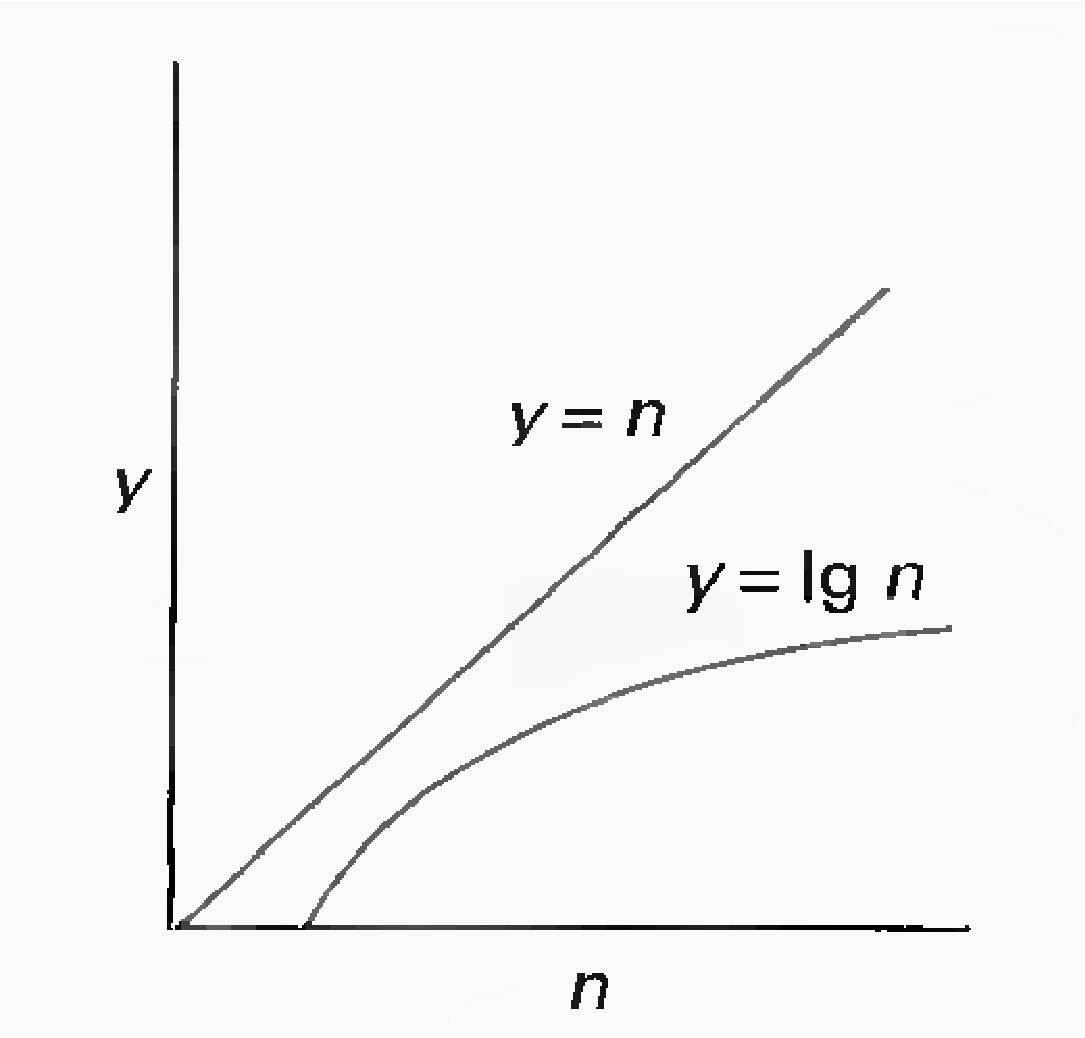
\includegraphics{ch7/fig1111.pdf}}
\label{fig:fig1111a}
}\qquad  \subfloat[ $n^2$ và $n \lg n$]{
  \scalebox{0.35}{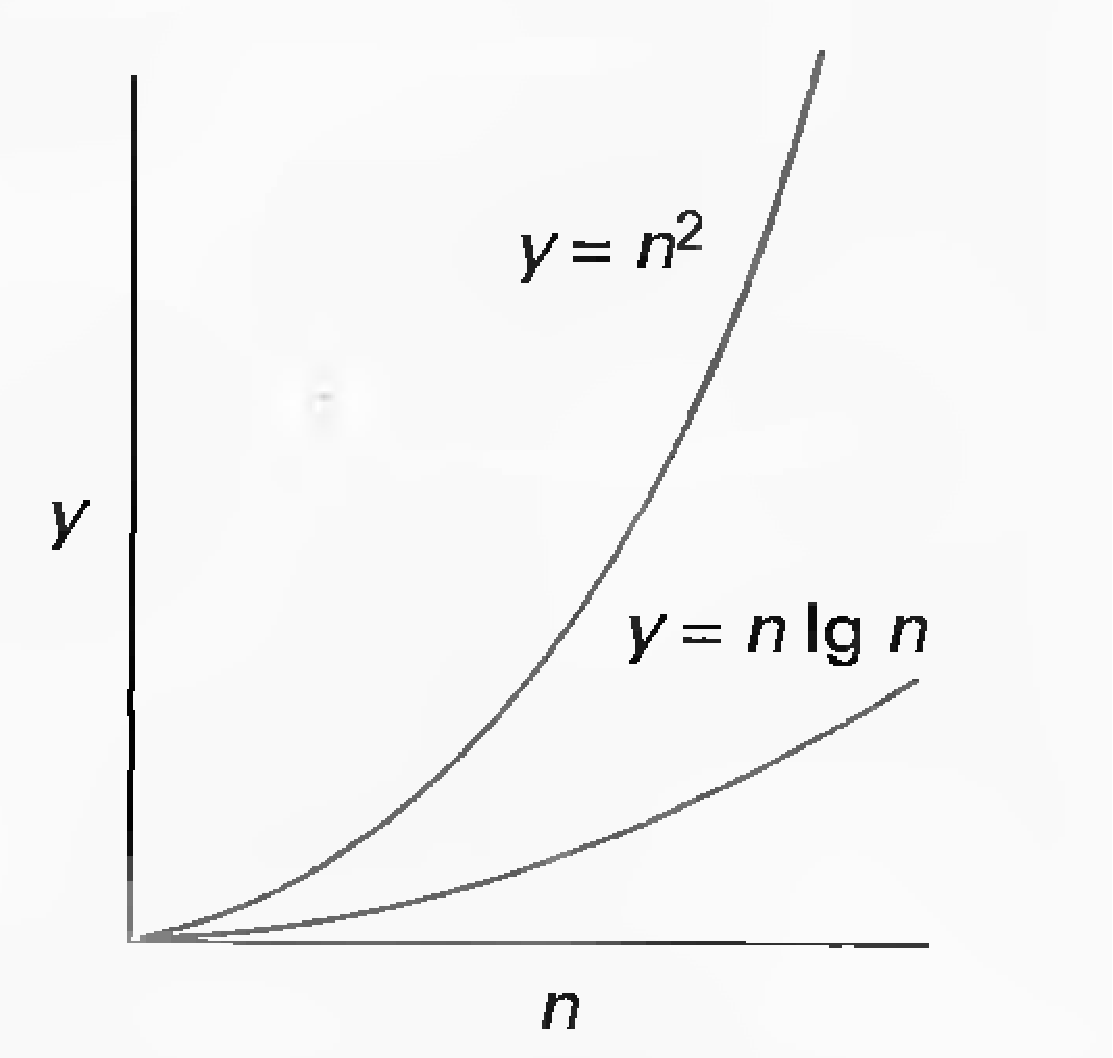
\includegraphics{ch7/fig1111b.pdf}}
\label{fig:fig1111b}
}  
\caption{Đồ thị của các hàm $n, \lg n, n \lg n,$ và $n^2$}
\end{figure}

Ta nói rằng một bài toán là \textbf{bài toán đa thức} nếu bài toán là $O(f(n))$, ở đó hàm
$f(n)$ hoặc là một đa thức hoặc bị chặn bởi một đa thức. Tập mọi bài toán đa thức được
biểu diễn bởi $\mathbf{P}$. Để ý rằng các thảo luận trước của ta chỉ ra rằng các bài toán
tìm kiếm danh sách và sắp xếp danh sách thuộc vào lớp $\mathbf{P}$.

Để nói rằng một bài toán là bài toán đa thức tức là khẳng định về thời gian yêu cầu để
giải bài toán đó. Ta thường nói rằng một bài toán trong $\mathbf{P}$ có thể được giải
trong thời gian đa thức hoặc bài toán có một lời giải trong thời gian đa thức.

Trong khoa học máy tính, việc xác định các bài toán thuộc vào lớp $\mathbf{P}$ là rất quan
trong bởi vì nó liên quan chặt chẽ đến các bài toán có lời giải chấp nhận được trong thực
tế. Thật vậy, các bài toán bên ngoài lớp $\mathbf{P}$ được đặc trưng như các bài toán có
thời gian chạy vô cùng lâu, thậm chí với đầu vào có kích thước nhỏ. Ta xem xét, ví dụ một
bài toán để tìm lời giải cần $2^n$ bước. Hàm $2^n$ rõ ràng không bị chặn bởi đa thức--nếu
$f(n)$ là một đa thức, vậy nếu ta tăng giá trị của $n$, ta sẽ thấy rằng các giá trị $2^n$
cuối cùng sẽ lớn hơn so với $f(n)$. Có nghĩa rằng một thuật toán với độ phức tạp
$\Theta(2^n)$ nói chũng sẽ ít hiệu quả, và bởi vậy nó yêu cầu nhiều thời gian hơn so với
một thuật toán với độ phức tạp $\Theta(f(n))$. Một thuật toán ở đó độ phức tạp là hàm mũ
được gọi là đòi hỏi thời gian mũ.

Ta xét một ví dụ cụ thể, là bài toán liệt kê mọi khả năng phân nhóm từ một tập có~$n$ phần
tử. Bởi vì có $2^n - 1$ cách phân nhóm (ta cho phép một nhóm có đủ tất cả mọi phần tử
nhưng không có phép nhóm không có phần tử nào), mọi thuật toán giải bài toán này cần ít
nhất $2^n - 1$ bước và bởi vậy độ phức tạp của nó ít nhất phải bằng với số này. Nhưng hàm
$2^n -1$ là hàm mũ, vậy nó không bị chặn bởi một đa thức. Bởi vậy mọi lời giải của bài
toán này tiêu tốn lượng thời gian vô cùng lớn nếu số phần tử của tập cần phân nhóm tăng
lên.

Ta thấy rằng bài toán phân nhóm có độ phức tạp lớn là do kích thước của đầu ra lớn. Tuy
nhiên, có tồn tại những bài toán độ phức tạp lớn thậm chí với đầu ra chỉ đơn thuần là câu
trả lời đơn giản có hay không. Một ví dụ là khả năng trả lời một câu hỏi về tính chân thực
của mệnh đề liên quan đến phép cộng các số thực. Ví dụ ta có thể nhận ra rằng câu hỏi ``có
tồn một số thực để tổng của nó với chính nó cho kết quả bằng $6$?'' có câu trả lời là có,
trong khi đó câu trả lời của câu hỏi ``có tồn tại một số thực khác không để tổng của nó
với chính nó bằng $0$?'' là không. Tuy vậy, khi câu hỏi phức tạp lên, ta sẽ gặp rất nhiều
khó khăn nếu muốn trả lời. Và nếu việc đối mặt với nhiều câu hỏi gợi ý cho ta rằng có thể
dùng máy tính để trợ giúp, thì không may, khả năng trả lời câu hỏi này đã được chứng minh
là đòi hỏi thời gian mũ, bởi thế, máy tính cuối cùng sẽ không thể trả lời câu hỏi này
trong thời gian cho phép khi câu hỏi phức tạp hơn.

Sự thật rằng các bài toán có thể giải được về mặt lý thuyết nhưng không ở
trong~$\mathbf{P}$ là có độ phức tạp thời gian vô cùng lớn đưa ta đến kết luận rằng các
bài toán này về cơ bản là không giải được trên thực tế. Các nhà khoa học máy tính gọi
chúng là các \textbf{bài toán bất trị}. Nói tóm lại, lớp $\mathbf{P}$ là một biên giới để
phân định bài toán nào là bất trị theo quan điểm thực tế. Bởi vậy nghiên cứu lớp
$\mathbf{P}$ là rất quan trọng đối với khoa học máy tính.

\subsection*{Bài toán NP}
Ta cùng xem xét \textbf{bài toán người bán hàng du lịch} (Travelling Salesman Problem, gọi
tắt là TSP). Yêu cầu của bài toán này là người bán hàng du lịch phải đi đến thăm từng
khách hàng của ở các thành phố khác nhau mà không được vượt quá ngân sách cho phép. Vấn đề
của anh ta là phải tìm một đường đi (bắt đầu từ nhà, đến các thành phố yêu cầu, rồi quay
về nhà) với độ dài đường đi không vượt quá số kilômét cho phép.

Lời giải cổ điển của bài toán này là xem xét một cách có hệ thống mọi đường đi có thể, và
so sánh độ dài của mỗi đường đi với số kilômét giới hạn cho tới khi tìm thấy một đường đi
chấp nhận được hoặc đã xem xét mọi khả năng. Cách tiếp cận này, tuy vậy không cho một lời
giải trong thời gian đa thức. Điều này là do khi số thành phố tăng lên, số các đường đi
phải kiểm tra tăng lên nhanh hơn so với mọi đa thức. Bởi vậy, việc giải bài toán TSP theo
cách này là không thực tế trong trường hợp số thành phố lớn.

Vậy muốn giải bài toán TSP trong thời gian chấp nhận được ta cần phải tìm một thuật toán
nhanh hơn. Giải pháp tham lam của ta là quan sát xem có một đường đi nào thoả mãn và sau
đó xem chuyện gì xảy ra nếu ta lựa chọn nó. Thuật toán này kết thúc rất nhanh chóng. Cụ
thể, danh sách các lệnh dưới đây có thể thực hiện nhanh chóng và có khả năng giải bài toán
này:
\begin{flushleft}
  \qquad     \textsl{Lấy một đường đi có thể, và tính toán khoảng cách của nó.} \\
  \qquad    \textsl{\textbf{If} (khoảng cách này không lớn hơn số kilômét cho phép)} \\
  \qquad    \textsl{\textbf{then} (thông báo thành công)} \\
  \qquad \textsl{\textbf{else} (thông báo không có)}
\end{flushleft}
Tuy nhiên, về mặt kỹ thuật dãy lệnh này không phải là một thuật toán. Lệnh đầu tiên là
nhập nhằng và ta không thể xác định đường đi nào được chọn hay không được chọn, và cũng
không xác định được làm thế nào có thể ra quyết định chọn. Thay vào đó nó cần đến sự sáng
tạo của cơ chế thực hiện chương trình để ra quyết định. Ta nói rằng các lệnh kiểu này là
không đơn định, và ta gọi một ``thuật toán'' chứa các lệnh kiểu này là \textbf{thuật toán
  không đơn định}.

Để ý rằng khi số các thành phố tăng lên, thời gian cần để thực hiện thuật toán không đơn
định ở trên tăng một cách chậm chạp. Quá trình lựa chọn một đường đi chỉ đơn thuần là đưa
ra một danh sách các thành phố, điều này có thể được làm trong khoảng thời gian tỉ lệ với
số các thành phố được yêu cầu. Hơn nữa, thời gian yêu cầu tính toán tổng khoảng cách trên
đường đi được chọn cũng tỉ lệ với số các thành phố được thăm, và thời gian yêu cầu để so
sánh tổng này với số kilômét giới hạn là độc lập với số thành phố. Nói tóm lại, thời gian
yêu cầu thực hiện thuật toán không đơn định này bị chặn bởi một đa thức. Bởi vậy ta có thể
giải bài toán TSP bởi một thuật toán không đơn định trong thời gian đa thức.

Tất nhiên, lời giải không đơn định của ta không thoả mãn về mặt tổng thể. Nó cần đến một
sự ước đoán may mắn. Nhưng sự tồn tại của nó lại gợi ý cho ta rằng có thể có một lời giải
đơn định của bài toán này chạy trong thời gian đa thức. Vấn đề thực sự có hay không một
thuật toán như vậy đến nay vẫn là một câu hỏi mở. Thực ra, bài toán TSP là một trong nhiều
bài toán được biết là có lời giải không đơn định chạy trong thời gian đa thức nhưng chưa
tìm thấy lời giải đơn định trong thời gian đa thức. Lời giải không đơn định trong thời
gian đa thức này làm ta hy vọng rằng một ngày nào đó sẽ tìm thấy một lời giải hiệu quả
thời gian đa thức. Tuy vậy, đến nay hầu hết mọi người đều tin rằng các bài toán kiểu này
là đủ phức tạp vượt ra ngoài khả năng của các thuật toán đơn định hiệu quả.

Bài toán có thể được giải trong thời gian đa thức bởi một thuật toán không đơn định được
gọi là một \textbf{bài toán đa thức không đơn định}, hay gọi tắt là \textbf{bài toán
  NP}. Ta thường ký hiệu lớp bài toán NP bằng $\mathbf{NP}$. Để ý rằng mọi bài toán trong
lớp $\mathbf{P}$ cũng thuộc $\mathbf{NP}$, bởi vì mọi thuật toán (đơn định) có thể thêm
một lệnh không đơn định vào mà không ảnh hưởng đến hiệu quả của chúng.

Tuy vậy câu hỏi có phải mọi bài toán NP cũng thuộc P vẫn là câu hỏi mở, như được chỉ ra
bởi bài toán TSP. Đây là bài toán chưa giải được nổi tiếng nhất trong khoa học máy tính
ngày nay. Lời giải của nó có rất nhiều ý nghĩa thực tế.

Trong nỗ lực giải quyết câu hỏi xem lớp $\mathbf{NP}$ có bằng $\mathbf{P}$ hay không,
người ta đã tìm thấy một lớp bài toán đặc biệt thuộc lớp $\mathbf{NP}$ gọi là các
\textbf{bài toán NP đầy đủ}. Các bài toán này có tính chất là nếu có một thuật toán thời
gian đa thức để giải một trong những bài toán này, thì sẽ có một thuật toán đơn định thời
gian đa thức để giải mọi bài toán khác trong lớp $\mathbf{NP}$; và vậy thì, lớp
$\mathbf{NP}$ trùng với lớp $\mathbf{P}$. Bài toán TSP là một ví dụ của một bài toán NP
đầy đủ.

\begin{figure}
  \centering
    \scalebox{0.3}{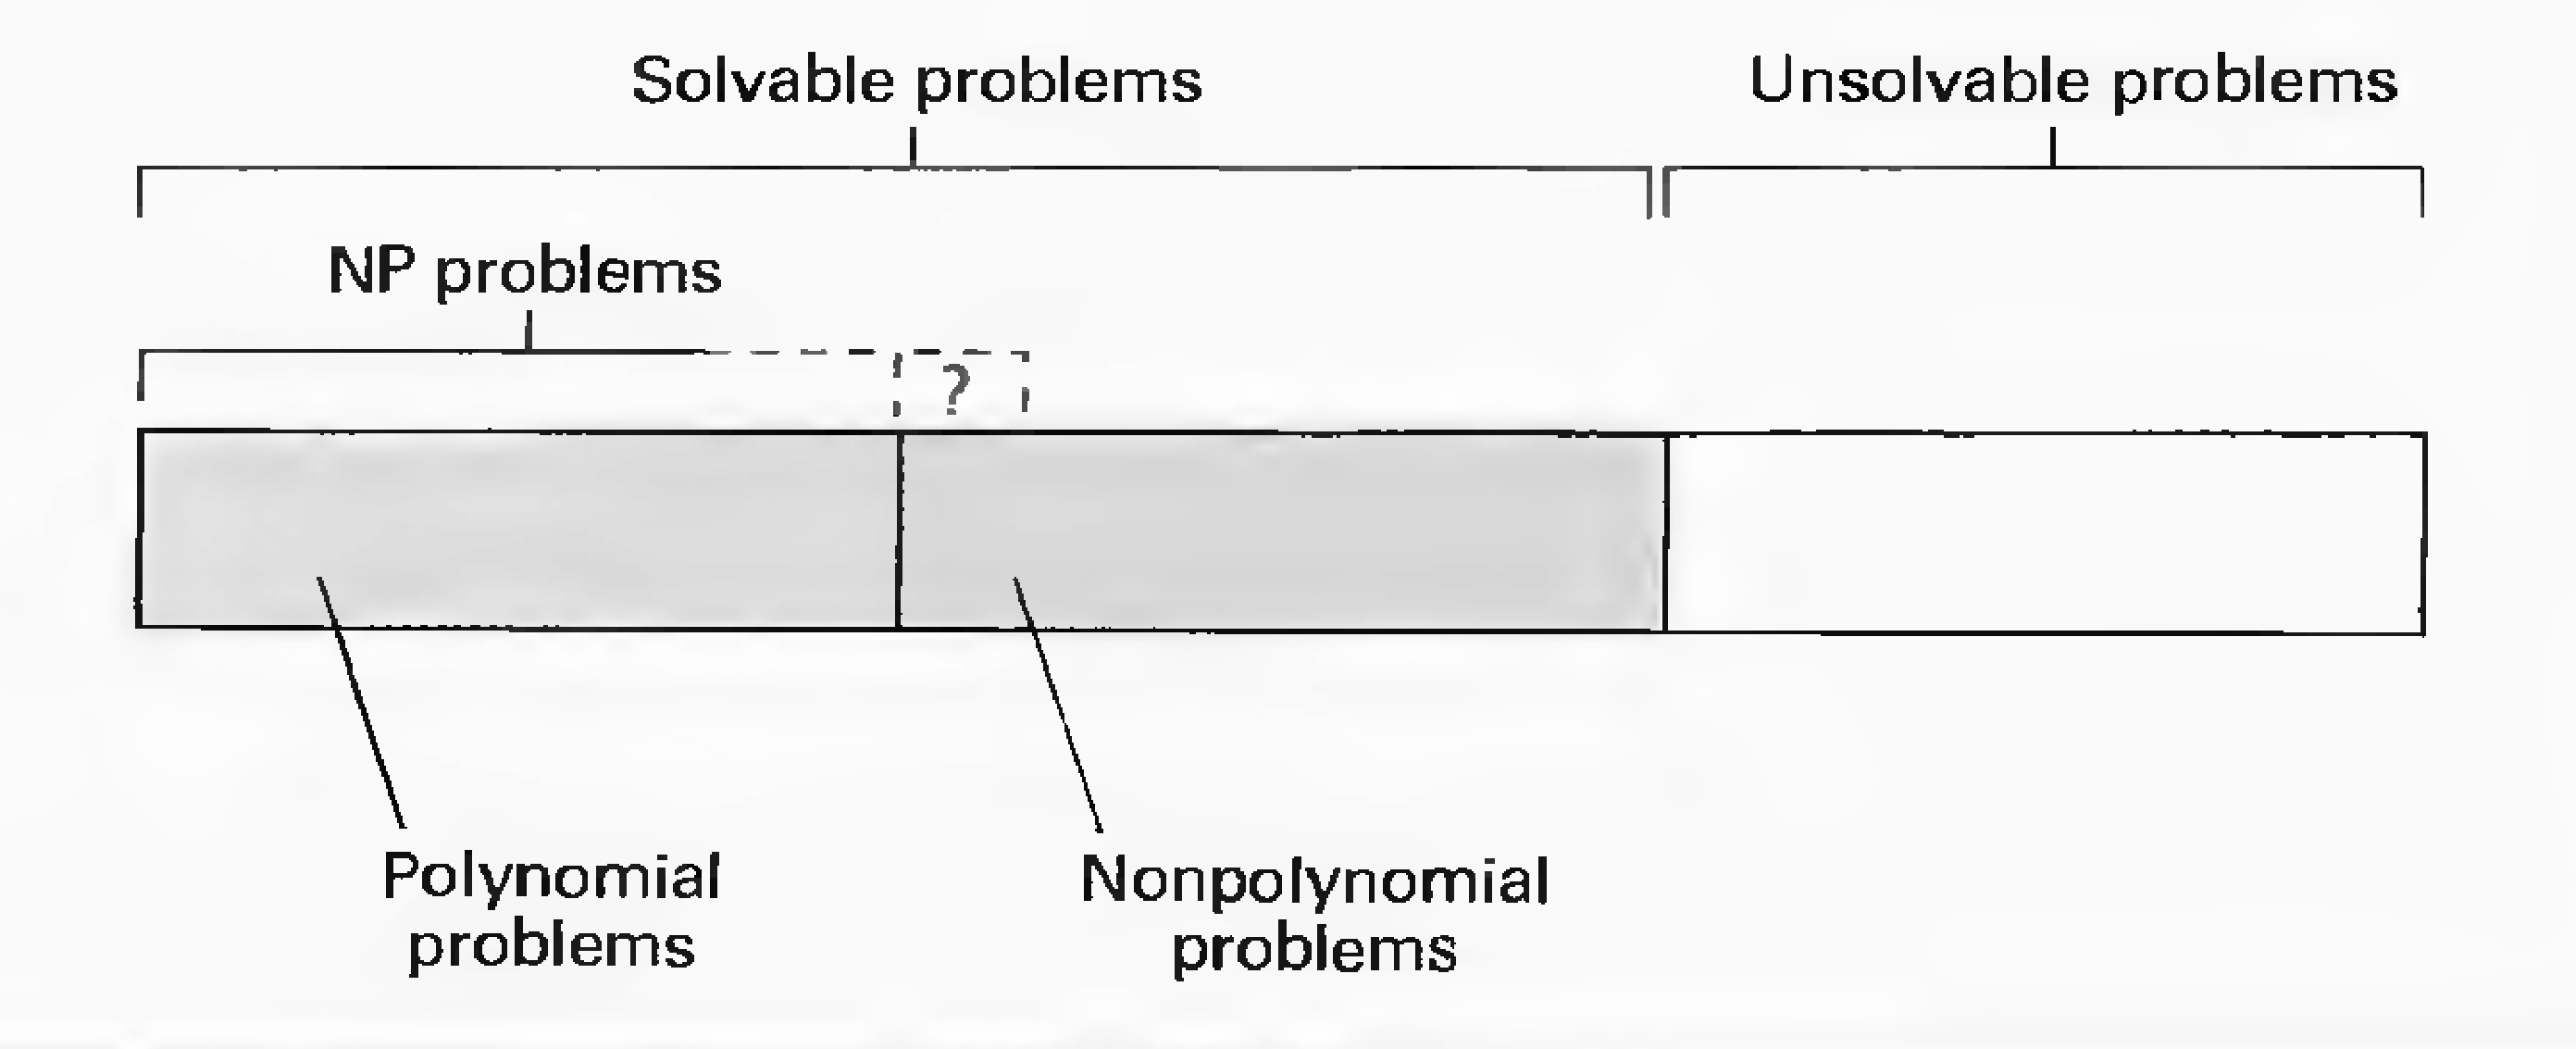
\includegraphics{ch7/fig1112.pdf}}
  \caption{Phân loại các lớp bài toán}
  \label{fig:fig1112}
\end{figure}

Tóm lại, một bài toán có thể phân loại thành hoặc giải được (có lời giải thuật toán) hoặc
không giải được (không có lời giải thuật toán), như được chỉ ra trong
Hình~\ref{fig:fig1112}. Hơn nữa, lớp các bài toán giải được lại được chia thành hai lớp
con. Một là lớp các bài toán thời gian đa thức, bao gồm các bài toán có lời giải chấp nhận
được trong thực tế. Hai là lớp các bài toán không đa thức, với các bài toán này lời giải
chấp nhận trong thực tế của chúng bị giới hạn với các đầu vào kích thước nhỏ và được lựa
chọn cẩn thận. Cuối cùng là lớp bài toán NP bí ẩn mà với hiểu biết hiện tại ta vẫn chưa
thể phân loại được.


\subsection*{Câu hỏi \& Bài tập}

\begin{enumerate}
\item Giả sử rằng một bài toán có thể giải được bởi một thuật toán trong $\Theta(2^n)$. Vậy
  ta có kết luận gì về độ phức tạp của bài toán này?

\item Giải sử một bài toán có thể được giải bởi một thuật toán trong $\Theta(n^2)$ và một
  thuật toán khác trong $\Theta(2^n)$. Thuật toán nào sẽ thực hiện tốt hơn?


\item Liệt kê mọi cách phân nhóm từ tập hai thành viên: Alice và Bill. Liệt kê mọi cách
  phân nhóm tập ba thành viên: Alice, Bill, và Carol. Liệt kê mọi cách phân nhóm của tập
  bốn thành viên: Alice, Bill, Carol, và David.


\item Hãy đưa ra một ví dụ về bài toán đa thức. Đưa ra một ví dụ về bài toán không đa
  thức. Đưa ra một ví dụ của về bài toán NP và chưa được chứng minh là bài toán đa thức.


\item Nếu độ phức tạp của thuật toán \texttt{X} lớn hơn độ phức tạp của thuật toán
  \texttt{Y}, có nhất thiết thuật toán \texttt{X} là khó hiểu hơn thuật toán \texttt{Y}?
  Hãy giải thích câu trả lời của bạn.
\end{enumerate}





%%% Local Variables: 
%%% mode: latex
%%% TeX-master: "../tindaicuong"
%%% End: 
